\documentclass{sig-alternate}
\usepackage{csquotes}
\usepackage{tikz}
\usetikzlibrary{matrix,shapes.multipart, arrows, shapes.geometric,fit,scopes}
\tikzset{
  >= latex,
  el/.style={ellipse, draw, text width=8em, align=center},
  rs/.style={rectangle split, draw, rectangle split parts=#1},
  ou/.style={draw, inner xsep=1em, inner ysep=1ex, fit=#1}
}

\newcommand{\lamine}[1]{\textbf{[Lamine: {\textcolor{red}{#1}}]}}
\newcommand{\laure}[1]{\textbf{[Laure: \textcolor{green}{#1}]}}
\newcommand{\tbd}[1]{\textbf{[TODO: \textcolor{blue}{#1}]}}

\begin{document}
\conferenceinfo{}{}

\title{Active Truth Finding for relevant Information Retrieval}

\numberofauthors{2} 
\author{
\alignauthor
Mouhamadou Lamine BA\\
       \affaddr{Qatar Computing Research Institute}\\
       \affaddr{Tornado Tower, West Bay}\\
       \affaddr{Doha, Qatar}\\
       \email{mlba@qf.org.qa}
% 2nd. author
\alignauthor
Laure Berti-Equille\\
       \affaddr{Qatar Computing Research Institute}\\
       \affaddr{Tornado Tower, West Bay}\\
       \affaddr{Doha; Qatar}\\
       \email{lberti.qf.org.qa}
%\and  % use '\and' if you need 'another row' of author names
}


\maketitle

% Page allocation for this demo
% 1.25 pages --> abstract + introduction
% 1.5 pages --> Active Truth finding Process
% 1 pages --> Demonstration system
% 0.25 pages --> references
\begin{abstract}
Open Web Information extraction systems like TextRunner~\cite{Yates07}
and popular Web search engines such as Google or Bind usually reply to
users' search queries by returning a set of potential relevant answers.
For some specific type of queries, the returned list might contain conflicting 
answers which make thing harder for the end-users to distinguish between the truth
and the false.
We demonstrate in the paper a system that processes answers outputted 
by open Web information extraction systems like TextRunner and provides 
the most probable answer together with corresponding trustworthy sources
using AllegatorTrack which is a system that implements a set of established
truth finding techniques. Our system has also the capability to account for users' feedbacks,
based on its knowledge of the correct instances for some searched relations, in order to improve
the truth finding process.
\end{abstract}

% A category with the (minimum) three required fields
%\category{H.4}{Information Systems Applications}{Miscellaneous}
%A category including the fourth, optional field follows...
%\category{D.2.8}{Software Engineering}{Metrics}[complexity measures, performance measures]

%\terms{Theory}

%\keywords{ACM proceedings, \LaTeX, text tagging}

% Introduction
\section{Introduction}
%\lamine{Page allocation}
%\begin{itemize}
 %\item 1.25 pages --> abstract + introduction
 %\item 1.5 pages --> Open information extraction + Active Ensembling for Truth Discovery 
 %\item 1 pages --> Demonstration System + Scenario
 %\item 0.25 pages --> References
%\end{itemize}

%\paragraph{Use cases}
%\begin{itemize}
% \item \textbf{Information extraction improvement:} Truth discovery over claims returned by OpenIE systems, e.g., TextRunner
% \item \textbf{Online hot news verification:} truth discovery over factual claims in each new's headline and
% content published on the online front page of AlJazeera
%\end{itemize}

Online fact-checkers such as FactCheck\footnote{FactCheck, {\small\url{ http://www.factcheck.org/}}}, Snopes\footnote{Snopes, {\small\url{ http://www.snopes.com/}}}, PolitiFact\footnote{PolitiFact,{\small \url{ http://www.politifact.com/}}}, TruthorFiction\footnote{TruthorFiction, {\small\url{ http://www.truthorfiction.com/}}} or OpenSecrets\footnote{OpenSecrets, {\small \url{ http://www.opensecrets.org/}}}) and ClaimBuster\footnote{ClaimBuster, {\small\url{ http://idir-server2.uta.edu/claimbuster}}} 
 have recently gained  unprecedented attention as their legitimate goal is to verify online information for enlightening public opinion and automate Web-scale fact-checking for assisting journalists \citep{Cohen2011,Hassan:2015}.
 However, estimating the veracity of data remains a challenging problem: extracting information from large, heterogeneous corpora of textual and multimedia documents and  integrating the extracted, multi-source data are difficult tasks. Data can be noisy, outdated, incorrect, conflicting, and thus unreliable, mainly due to information extraction errors,  low source quality and disagreements between the information sources. 
 
 [ ici: point sur etat de l'art des methods de truth discovery et nécessité de faire ensembling car one-fits-all solution does not exist for open  domain + nécessité d'intégrer/developper full truth discovery pipeline incluant l'extraction]
 
In this demo, we present {\scschape Vera}, a web-platform that supports information extraction, data fusion, truth finding, and visualization of large-scale, multisource data from the Web.

The main contributions of our work are:

 [ici: lister contrib]
 
 
{\scschape Vera} platform, REST API and additional information, data sets and material are available at \url{dafna.qcri.org}.


 


% Active Truth Finding for relevant information search
% Active Ensembling for Truth Finding
\subsection{Truth Discovery}\label{truthfinding}
$\VERA$ supports an adaptive truth discovery approach based on ensembling and active learning to compute the optimal labeling and scoring results from a set of truth discovery algorithms. Our approach outperforms individual truth discovery technique on any given data set. It actively leverages the user's knowledge when available for finding the true claims and update the trustworthiness score of the sources. When user's knowledge or training data are not available, $\VERA$ still provides meaningful results using ensembling of methods with minimizing the disagreement between methods.

\noindent{\bf Competing Classifiers.} 
In our context, the truth discovery algorithms are considered as  binary classifiers whose goal is to label each conflicting value as a true or false answer to the user query.

$\VERA$ integrates and combines  twelve state-of-the art truth discovery algorithms that can be classified in three categories as follows:
\begin{inparaenum}[(1)]
\item Agreement-based methods including  TruthFinder~\cite{YinHY08}, Cosine, 2-Estimates and 3-Estimates~\cite{GallandAMS10}, AccuNoDep~\cite{DongBS09}; 
\item MAP Estimation-based methods including  MLE~\cite{WangKLA12}, LTM~\cite{ZhaoRGH12}, SimpleLCA and GuessLCA~\cite{PasternackR13}; and
 \item Bayesian Inference-based methods including  Depen, Accu, and AccuSim~\cite{DongBS09}.
\end{inparaenum}



\noindent{\bf Ensembling.} 
\label{ensembling} Ensembling is a semi-supervised learning approach  combining various competing models that has been demonstrated to be very effective in many disciplines~\cite{Burr12}. $\VERA$ ensembling method discovers the optimal set (ensemble) of classifiers for the truth discovery classification problem by actively learning from an oracle, e.g., the user or a reference model over a sample of data. Ensembling  enables to perform
classification consistently well across various data sets without having to determine \emph{a priori} a suitable classifier 
type.  $\VERA$ exploits ensembling for combining truth discovery methods in the two following cases:
\begin{inparaenum}[(1)]
\item  When the user can provide either \emph{a priori} or \emph{a posteriori} truth labels for few claims as instances of the ground truth (under a limited budget and with expected guarantees); 
\item When no ground truth training data are available.
\end{inparaenum}

In the first case, $\VERA$  actively learns from the user's labels over the training data, finds the best ensemble of classifiers and returns the veracity labels and scores for the rest of the data. 

In the second case, $\VERA$ selects the candidate ensembling which satisfies our time-dependent consensus model. This model captures three intuitive ideas: 
\begin{inparaenum}[(i)]
\item Initially, very few sources with diverse authoritativeness degrees may observe an event and report information  (e.g., in case of disaster or  bombing). As long as the information is  not confirmed (or denied)  by a sufficient number of other independent sources, unknown or non-reputable  sources should not be penalized and the authoritativeness of the sources should not influence the veracity estimation;
\item The number of conflicting information claimed by multiple sources has a decreasing variability in time; and
\item  The majority of sources cannot be trusted until a certain time-point where a consensus on the fact (i.e., the true value) is reached as illustrated in Figure 2.
\end{inparaenum}

Truth discovery is hard in practical scenarios because there is often no prior ground truth guiding
the selection of an algorithm, in particular when the context is dynamic. More importantly, a large set of labeled 
data (or training data) is generally out-of-reach in the context of Web and social media data. As a consequence, it remains usually
hard to evaluate the precision/recall of existing algorithms on real-world data. %

However, users may have background knowledge about some real-world facts or about the reliability of particular sources. Such knowledge can be very valuable not only \emph{a priori} for guiding $\VERA$ truth discovery computation, but also \emph{a posteriori} 
for evaluating and backtracking the errors.

In our demonstration scenarios, we will show the two operational modes of $\VERA$ which combines truth discovery and open information extraction with ensemble-based active learning for estimating data veracity with  and without prior knowledge of the user, also learning from posterior knowledge in order to improve the next truth discovery computations.% 

\subsection{Result Exploration}\label{visu}
$\VERA$ features a layer for result visualization and explanation
basically consisting of a set of Web user interfaces (panels and
option widgets) and decision algorithms which respectively enable
 viewing and browsing the truth discovery results 
  to obtain more deeper insights and understand 
how the estimation of the veracity of each claim has been computed
by the system. This layer also provides the ability to input truth
labels for a limited subset of claims. Explanation is accomplished
in $\VERA$ through APIs whereas result visualization
renders the output of the truth discovery process to ease
user exploration and interaction with the system, as we will detail hereafter.


\noindent{\bf Visualization.}
$\VERA$ currently supports three artifacts to visualize
and browse  the results of query answering. When a  user query is submitted to $\VERA$,
candidate claims are extracted and truth discovery computation is performed. 
A list-based artifact then presents the candidate
answers to the user. For each object property 
related to the user query, the candidate answers are ranked
 in a decreasing order of veracity scores, 
 i.e., the answer with the highest veracity score (the most likely to be true) is listed
first, then the answer with the second highest veracity score is given,
and so on. Each  line of the result list contains a claimed
answer, its  veracity score and label (\url{True} or \url{False})
returned by the Truth Discovery layer, with the option widget to view 
the set of sources supporting it (\url{view_sources}), and an illustrative
excerpt from the content of the Web document or tweet from which the answer has
been extracted. Candidate claims are presented to the user with an
additional widget option \url{user_input_label} that enables the user
to eventually propose a labelling or add background knowledge. 
For further result exploration, $\VERA$ 
has set two other visualization artifacts. Indeed, when the user
chooses the option widget \url{view_sources}, $\VERA$  presents the
complete list of sources which support the corresponding claim, their
trustworthiness scores computed by the Truth Discovery layer, and their
associated corpus. Finally, the user can access to the explanation
window to better understand the  estimation of the veracity
score of a particular answer by clicking on it.


\noindent{\bf Explanation.}
$\VERA$ relies on DAFNA API \cite{Wagui15} to generate explanations for the results of the truth discovery process. 
It is accessible via its endpoint \textbf{runs}. Given a claim identifier, the system can explain how the returned score of veracity has been
computed using the  ensemble of truth discovery algorithms. %

To this end, DAFNA builds an explanation decision tree representing the different
choices made by the ensemble applied to the candidate answers. 
Every decision tree is  built from the
number of supporting vs. disagreeing sources,  their trustworthy levels, and the set of conflicting values. $\VERA$ leverages the explanation functionality of DAFNA  to provide insights of the results when requested by the
user.



% Demonstration system
\section{Our Demonstration System}\label{demonstration}
We describe in this section our system for 
combining truth discovring and information
extraction with active ensembling using the procedure described
in the previous sections. We first 
present the architecture of our system by
giving its different modules. Then, we provide
a typical demonstration scenario of a user interacting
with our system.


% Architecture and GUI
\subsection{System Components}
The architecture of our demonstration system, given in
Figure~\ref{system_architecture}, comprises the following
five main components.

% User I/O Interface
\paragraph*{User Interface}
The user interface is the main component that enables a given user 
to interact with our system. Via the user interface component, 
one has the ability to provide a query (or a key phrase), to
recieve answers from the truth finding module or  label requests
from the active ensembling module. When a label request is sent 
is sent to the user, she (or he) also provides his answers through 
this component.


% Information extraction module
\paragraph*{OpenIE component} OpenIE is responsible to the extraction 
of information from the Web. It considers, as an input, a user query and queries
several Web corpus in order to returns the relevant set of candidate answers. Our
OpenIE component relies on TextRunner engine for the extraction of the set of candidate
Web claims with respect to a user query about a given real-world fact.

% Learning module
\paragraph*{Active Ensembling Module} This is the core component of our system which discovers
an optimal ensemble for truth finding over candidate claims extracted with the OpenIE 
component. The active ensembling module, as described in Section~3, evaluates set of twelves
truth finding algorithms on unlabeled claims, figures out the most controversal claims, and requests
labels from the user. Once it obtained feebacks from the user, it estimates the accuracy of the competing
algorithms on the labeled claims, and finally decides about the best one to use for each set of claims related 
to the same query or fact. The module returns an ensemble since one can have distinct good truth finding techniques
for various sets of claims about different facts.

% Truth finding engine
\paragraph*{Truth Finding Module} It corresponds to AllegatorTrack which contains
twelve truth finding algorithms with different accuracy according to the types of 
claims and the characteristics of sources.



% knwoledge bases
\paragraph*{Storage Module}The knowledge base contains the information used for the learning
phase the truth finding procedure. These information include the true facts for some relations
which have been learnt based on the feedbacks of the users. In addition, our knowledge base could
be enriched with ground truth about some facts from reliable sources such as Wikipedia. Based on 
the knowledge base, our system has the ability to improve the accuracy of the truth finding process
by learning about the best method to use or the best parameters, e.g., sources' accuracy scores, to 
consider for a better boostrapping of the process.

\begin{figure}[ht]
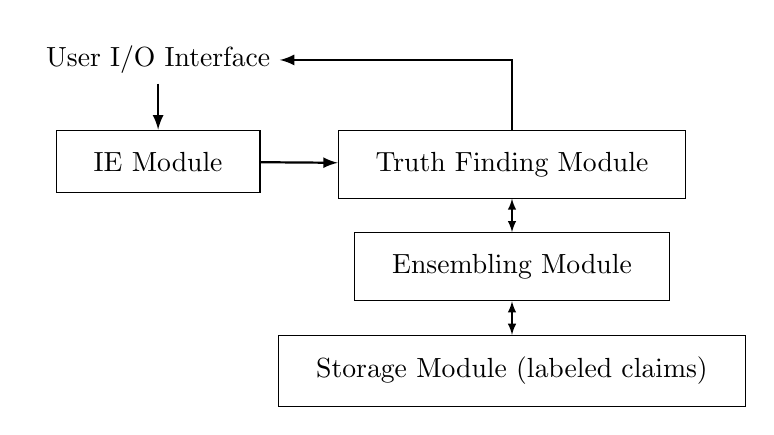
\begin{tikzpicture}[auto, line/.style ={draw,  thick, shorten <=0pt}]
  \matrix[matrix of nodes, row sep=5ex, column sep=1em] (mx) {
    User I/O Interface &\\
    IE Module &  Truth Finding Module\\
    & Ensembling Module\\ 
    & Storage Module (labeled claims)\\
  };
  %\node[ou=(mx-1-3)] (empty) {};
  \node[ou=(mx-2-1)] (oi) {};
  \node[ou=(mx-2-2)] (tf) {};
  \node[ou=(mx-3-2)] (lm) {};
  \node[ou=(mx-4-2)] (kb) {};
  %{[->, thick]
  %\draw(mx-1-1)edge(empty);
  %}
  {[->, thick]
  \draw(mx-1-1)edge(oi);
  \draw(oi)edge(tf);
  }
  {[<->]
    \draw(tf)edge(lm);
     \draw(lm)edge(kb);
  }
  \begin{scope}[every path/.style=line, <-]
   \path(mx-1-1)  - | (tf);
  % \path(mx-1-3)  - | (lm);
  \end{scope}

\end{tikzpicture}
\caption{Architecture of our system}\label{system_architecture}
\end{figure}
% Demonstration scenario
\subsection{Demonstration scenario}
A given user that wants to interact with our system
must do it through the search form. Through the search
form, she (or he) provides her searched relation, e.g.,
``Where is born Barack Obama?".
The searched relation is then 
passed to the information extraction engine,  TextRunner system
in our case, which returns a set of answers considered to be 
relevant for the user's request. Each claim in the returned list is
processed in order to extract the corresponding sources along a detailed
description of the claim which we format in a certain manner. The 
set of sources and the formatted versions of all claims are then passed
to the truth finding module which integrate all the claims and compute the
most probable answer together with the reliability scores of participated 
sources for the searched relation. Finally, the output of the truth finding
process is returned to the user. The user can also want to review the output
of our system by definitively validiting it or not through its knwoledge of the
modeled world. For example when the system has totally wrong, it may be interesting
to get such a kind of feedbacks from the user in order to change the used method, as
there are many available with our system, and to enhance the process for the further 
search about the same world. The user gives feedbacks using the option buttons on the 
left-hand side of the outputted claims or the text form. The feebacks given by the user
is saved in knwoledge bases within our system for further processes.


% Conclusion
\section{Conclusion}
% References
\cite{*}
\bibliographystyle{plain}
\bibliography{biblio}

\end{document}
